\documentclass[twoside]{book}

% Packages required by doxygen
\usepackage{fixltx2e}
\usepackage{calc}
\usepackage{doxygen}
\usepackage{graphicx}
\usepackage[utf8]{inputenc}
\usepackage{makeidx}
\usepackage{multicol}
\usepackage{multirow}
\PassOptionsToPackage{warn}{textcomp}
\usepackage{textcomp}
\usepackage[nointegrals]{wasysym}
\usepackage[table]{xcolor}

% Font selection
\usepackage[T1]{fontenc}
\usepackage{mathptmx}
\usepackage[scaled=.90]{helvet}
\usepackage{courier}
\usepackage{amssymb}
\usepackage{sectsty}
\renewcommand{\familydefault}{\sfdefault}
\allsectionsfont{%
  \fontseries{bc}\selectfont%
  \color{darkgray}%
}
\renewcommand{\DoxyLabelFont}{%
  \fontseries{bc}\selectfont%
  \color{darkgray}%
}
\newcommand{\+}{\discretionary{\mbox{\scriptsize$\hookleftarrow$}}{}{}}

% Page & text layout
\usepackage{geometry}
\geometry{%
  a4paper,%
  top=2.5cm,%
  bottom=2.5cm,%
  left=2.5cm,%
  right=2.5cm%
}
\tolerance=750
\hfuzz=15pt
\hbadness=750
\setlength{\emergencystretch}{15pt}
\setlength{\parindent}{0cm}
\setlength{\parskip}{0.2cm}
\makeatletter
\renewcommand{\paragraph}{%
  \@startsection{paragraph}{4}{0ex}{-1.0ex}{1.0ex}{%
    \normalfont\normalsize\bfseries\SS@parafont%
  }%
}
\renewcommand{\subparagraph}{%
  \@startsection{subparagraph}{5}{0ex}{-1.0ex}{1.0ex}{%
    \normalfont\normalsize\bfseries\SS@subparafont%
  }%
}
\makeatother

% Headers & footers
\usepackage{fancyhdr}
\pagestyle{fancyplain}
\fancyhead[LE]{\fancyplain{}{\bfseries\thepage}}
\fancyhead[CE]{\fancyplain{}{}}
\fancyhead[RE]{\fancyplain{}{\bfseries\leftmark}}
\fancyhead[LO]{\fancyplain{}{\bfseries\rightmark}}
\fancyhead[CO]{\fancyplain{}{}}
\fancyhead[RO]{\fancyplain{}{\bfseries\thepage}}
\fancyfoot[LE]{\fancyplain{}{}}
\fancyfoot[CE]{\fancyplain{}{}}
\fancyfoot[RE]{\fancyplain{}{\bfseries\scriptsize Generated on Thu Jun 16 2016 16\+:53\+:43 for Lame\+Wireframe by Doxygen }}
\fancyfoot[LO]{\fancyplain{}{\bfseries\scriptsize Generated on Thu Jun 16 2016 16\+:53\+:43 for Lame\+Wireframe by Doxygen }}
\fancyfoot[CO]{\fancyplain{}{}}
\fancyfoot[RO]{\fancyplain{}{}}
\renewcommand{\footrulewidth}{0.4pt}
\renewcommand{\chaptermark}[1]{%
  \markboth{#1}{}%
}
\renewcommand{\sectionmark}[1]{%
  \markright{\thesection\ #1}%
}

% Indices & bibliography
\usepackage{natbib}
\usepackage[titles]{tocloft}
\setcounter{tocdepth}{3}
\setcounter{secnumdepth}{5}
\makeindex

% Hyperlinks (required, but should be loaded last)
\usepackage{ifpdf}
\ifpdf
  \usepackage[pdftex,pagebackref=true]{hyperref}
\else
  \usepackage[ps2pdf,pagebackref=true]{hyperref}
\fi
\hypersetup{%
  colorlinks=true,%
  linkcolor=blue,%
  citecolor=blue,%
  unicode%
}

% Custom commands
\newcommand{\clearemptydoublepage}{%
  \newpage{\pagestyle{empty}\cleardoublepage}%
}


%===== C O N T E N T S =====

\begin{document}

% Titlepage & ToC
\hypersetup{pageanchor=false,
             bookmarks=true,
             bookmarksnumbered=true,
             pdfencoding=unicode
            }
\pagenumbering{roman}
\begin{titlepage}
\vspace*{7cm}
\begin{center}%
{\Large Lame\+Wireframe \\[1ex]\large 1.\+0 }\\
\vspace*{1cm}
{\large Generated by Doxygen 1.8.8}\\
\vspace*{0.5cm}
{\small Thu Jun 16 2016 16:53:43}\\
\end{center}
\end{titlepage}
\clearemptydoublepage
\tableofcontents
\clearemptydoublepage
\pagenumbering{arabic}
\hypersetup{pageanchor=true}

%--- Begin generated contents ---
\chapter{License}
\label{License}
\hypertarget{License}{}
This library is free software\+: you can redistribute it and/or modify it under the terms of the G\+N\+U Lesser General Public License as published by the Free Software Foundation, either version 3 of the License, or (at your option) any later version.

This program is distributed in the hope that it will be useful, but W\+I\+T\+H\+O\+U\+T A\+N\+Y W\+A\+R\+R\+A\+N\+T\+Y; without even the implied warranty of M\+E\+R\+C\+H\+A\+N\+T\+A\+B\+I\+L\+I\+T\+Y or F\+I\+T\+N\+E\+S\+S F\+O\+R A P\+A\+R\+T\+I\+C\+U\+L\+A\+R P\+U\+R\+P\+O\+S\+E. See the G\+N\+U Lesser General Public License for more details.

You should have received a copy of the G\+N\+U Lesser General Public License along with this program. If not, see \href{http://www.gnu.org/licenses/}{\tt http\+://www.\+gnu.\+org/licenses/}. 
\chapter{Hierarchical Index}
\section{Class Hierarchy}
This inheritance list is sorted roughly, but not completely, alphabetically\+:\begin{DoxyCompactList}
\item \contentsline{section}{driedobj}{\pageref{classdriedobj}}{}
\item \contentsline{section}{Edge}{\pageref{structEdge}}{}
\item \contentsline{section}{Vertex}{\pageref{structVertex}}{}
\item window\begin{DoxyCompactList}
\item \contentsline{section}{hwlib\+:\+:bufferwindow}{\pageref{classhwlib_1_1bufferwindow}}{}
\end{DoxyCompactList}
\end{DoxyCompactList}

\chapter{Data Structure Index}
\section{Data Structures}
Here are the data structures with brief descriptions\+:\begin{DoxyCompactList}
\item\contentsline{section}{\hyperlink{classhwlib_1_1bufferwindow}{hwlib\+::bufferwindow} \\*Main class of dubblebufferd, a decorator for hwlib windows }{\pageref{classhwlib_1_1bufferwindow}}{}
\item\contentsline{section}{\hyperlink{classdriedobj}{driedobj} \\*The main class, it can manipulate and draw 3d objects }{\pageref{classdriedobj}}{}
\item\contentsline{section}{\hyperlink{structEdge}{Edge} \\*\hyperlink{structEdge}{Edge} struct to connect 2 Vertexes }{\pageref{structEdge}}{}
\item\contentsline{section}{\hyperlink{structVertex}{Vertex} \\*\hyperlink{structVertex}{Vertex} structure to store 3\+D coordinates }{\pageref{structVertex}}{}
\end{DoxyCompactList}

\chapter{File Index}
\section{File List}
Here is a list of all documented files with brief descriptions\+:\begin{DoxyCompactList}
\item\contentsline{section}{Arduino\+\_\+implementation/\+Lib/3\+D lib/\hyperlink{ddd_8cpp}{ddd.\+cpp} }{\pageref{ddd_8cpp}}{}
\item\contentsline{section}{Arduino\+\_\+implementation/\+Lib/3\+D lib/\hyperlink{ddd_8hpp}{ddd.\+hpp} \\*3\+D header }{\pageref{ddd_8hpp}}{}
\item\contentsline{section}{Arduino\+\_\+implementation/\+Lib/\+Dubblebufferlib/\hyperlink{hwlib-dubblebufferd_8hpp}{hwlib-\/dubblebufferd.\+hpp} \\*Double bufferd Hwlib header, can be used as an extension to hwlib }{\pageref{hwlib-dubblebufferd_8hpp}}{}
\item\contentsline{section}{Arduino\+\_\+implementation/\+Lib/\+Mathlib/\hyperlink{easymath_8h}{easymath.\+h} \\*My optimized math library, greatly inspired and influenced by the work of Oscar Liang and the Speed\+Trig math library }{\pageref{easymath_8h}}{}
\end{DoxyCompactList}

\chapter{Data Structure Documentation}
\hypertarget{classhwlib_1_1bufferwindow}{\section{hwlib\+:\+:bufferwindow Class Reference}
\label{classhwlib_1_1bufferwindow}\index{hwlib\+::bufferwindow@{hwlib\+::bufferwindow}}
}


the main class of dubblebufferd, a decorator for hwlib windows.  




{\ttfamily \#include $<$hwlib-\/dubblebufferd.\+hpp$>$}



Inheritance diagram for hwlib\+:\+:bufferwindow\+:
\nopagebreak
\begin{figure}[H]
\begin{center}
\leavevmode
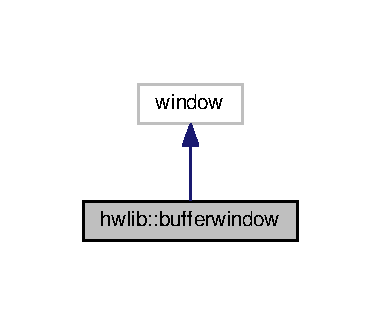
\includegraphics[width=183pt]{classhwlib_1_1bufferwindow__inherit__graph}
\end{center}
\end{figure}


Collaboration diagram for hwlib\+:\+:bufferwindow\+:
\nopagebreak
\begin{figure}[H]
\begin{center}
\leavevmode
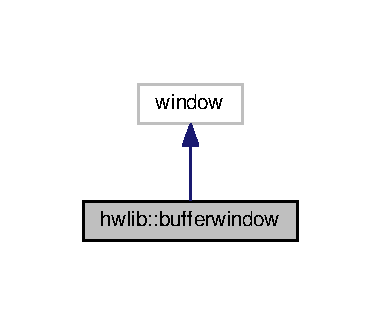
\includegraphics[width=183pt]{classhwlib_1_1bufferwindow__coll__graph}
\end{center}
\end{figure}
\subsection*{Public Member Functions}
\begin{DoxyCompactItemize}
\item 
\hyperlink{classhwlib_1_1bufferwindow_ab7b3cae85b441cfc9123201b30b86dae}{bufferwindow} (window \&slave\+Window)
\begin{DoxyCompactList}\small\item\em The decorator of a buffered window. \end{DoxyCompactList}\item 
\hypertarget{classhwlib_1_1bufferwindow_abfe7d7caa932892ca025d1dab49b13d4}{virtual void {\bfseries clear} ()}\label{classhwlib_1_1bufferwindow_abfe7d7caa932892ca025d1dab49b13d4}

\item 
\hypertarget{classhwlib_1_1bufferwindow_aa25f7a689ad5328e457c963b7a348d81}{void {\bfseries flush} ()}\label{classhwlib_1_1bufferwindow_aa25f7a689ad5328e457c963b7a348d81}

\end{DoxyCompactItemize}


\subsection{Detailed Description}
the main class of dubblebufferd, a decorator for hwlib windows. 

This class implements an decorator to any$\ast$ hwlib window, it adds the functionallity of dubble buffering for windows that take a very long time to clear and rewrite completly each frame, such as S\+S\+D1306 controlled screens. right now I only support the S\+S\+D1306 Glcd-\/\+Oled window because that is \#1 priority

It uses an array of bools instead of working with bitwise operators because the memory loss outweighed the performance increase, plus it was way easier to make in my available time.

Usage\+: The only thing you need to change in your code is add a .flush() command every time you want to update the screen 

\subsection{Constructor \& Destructor Documentation}
\hypertarget{classhwlib_1_1bufferwindow_ab7b3cae85b441cfc9123201b30b86dae}{\index{hwlib\+::bufferwindow@{hwlib\+::bufferwindow}!bufferwindow@{bufferwindow}}
\index{bufferwindow@{bufferwindow}!hwlib\+::bufferwindow@{hwlib\+::bufferwindow}}
\subsubsection[{bufferwindow}]{\setlength{\rightskip}{0pt plus 5cm}hwlib\+::bufferwindow\+::bufferwindow (
\begin{DoxyParamCaption}
\item[{window \&}]{slave\+Window}
\end{DoxyParamCaption}
)\hspace{0.3cm}{\ttfamily [inline]}}}\label{classhwlib_1_1bufferwindow_ab7b3cae85b441cfc9123201b30b86dae}


The decorator of a buffered window. 


\begin{DoxyParams}{Parameters}
{\em slave\+Window} & slave\+Window is a reference to any hwlib window. \\
\hline
\end{DoxyParams}


The documentation for this class was generated from the following file\+:\begin{DoxyCompactItemize}
\item 
Arduino\+\_\+implementation/\+Lib/\+Dubblebufferlib/\hyperlink{hwlib-dubblebufferd_8hpp}{hwlib-\/dubblebufferd.\+hpp}\end{DoxyCompactItemize}

\hypertarget{classdriedobj}{\section{driedobj Class Reference}
\label{classdriedobj}\index{driedobj@{driedobj}}
}


The main class, it can manipulate and draw 3d objects.  




{\ttfamily \#include $<$ddd.\+hpp$>$}



Collaboration diagram for driedobj\+:
\nopagebreak
\begin{figure}[H]
\begin{center}
\leavevmode
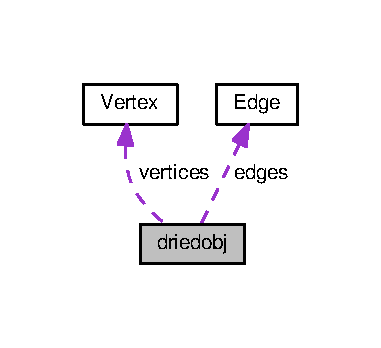
\includegraphics[width=183pt]{classdriedobj__coll__graph}
\end{center}
\end{figure}
\subsection*{Public Member Functions}
\begin{DoxyCompactItemize}
\item 
\hyperlink{classdriedobj_afb127c8b8fb3eeccac0b10223058a454}{driedobj} (hwlib\+::window \&w, \hyperlink{structVertex}{Vertex} vertices\mbox{[}$\,$\mbox{]}, \hyperlink{structEdge}{Edge} edges\mbox{[}$\,$\mbox{]}, unsigned char verticelength, unsigned char edgelength, unsigned int screenwidth, unsigned int screenheight)
\begin{DoxyCompactList}\small\item\em This is the decorator of the main class, it is a 3d object you can draw on 2d windows. \end{DoxyCompactList}\item 
\hypertarget{classdriedobj_a7f650e57daea2e35095554131718d088}{void \hyperlink{classdriedobj_a7f650e57daea2e35095554131718d088}{rotate\+X} (float degrees)}\label{classdriedobj_a7f650e57daea2e35095554131718d088}

\begin{DoxyCompactList}\small\item\em Rotate the object over the X-\/axis with x amount of degrees. \end{DoxyCompactList}\item 
\hypertarget{classdriedobj_a7ec55d1803e85e6dab3fe23c9f387d98}{void \hyperlink{classdriedobj_a7ec55d1803e85e6dab3fe23c9f387d98}{rotate\+Y} (float degrees)}\label{classdriedobj_a7ec55d1803e85e6dab3fe23c9f387d98}

\begin{DoxyCompactList}\small\item\em Rotate the object over the Y-\/axis with x amount of degrees. \end{DoxyCompactList}\item 
\hypertarget{classdriedobj_a7d23752e964832477cc266605ee4234f}{void \hyperlink{classdriedobj_a7d23752e964832477cc266605ee4234f}{rotate\+Z} (float degrees)}\label{classdriedobj_a7d23752e964832477cc266605ee4234f}

\begin{DoxyCompactList}\small\item\em Rotate the object over the Z-\/axis with x amount of degrees. \end{DoxyCompactList}\item 
\hypertarget{classdriedobj_a1dd0bfeb6d88453a057f759b7f969bbe}{void \hyperlink{classdriedobj_a1dd0bfeb6d88453a057f759b7f969bbe}{translate} (float x, float y, float z)}\label{classdriedobj_a1dd0bfeb6d88453a057f759b7f969bbe}

\begin{DoxyCompactList}\small\item\em Translate the object (move it around the world) by adding or subtracting its x y and z coordinates. \end{DoxyCompactList}\item 
\hypertarget{classdriedobj_a30f12a90a332520104c379ca48ca5e55}{void \hyperlink{classdriedobj_a30f12a90a332520104c379ca48ca5e55}{scale} (float scale)}\label{classdriedobj_a30f12a90a332520104c379ca48ca5e55}

\begin{DoxyCompactList}\small\item\em Scale the object to make it bigger or smaller. \end{DoxyCompactList}\item 
\hypertarget{classdriedobj_a1ff67fb7a91ebaefbb5073d296411c3c}{void \hyperlink{classdriedobj_a1ff67fb7a91ebaefbb5073d296411c3c}{draw} ()}\label{classdriedobj_a1ff67fb7a91ebaefbb5073d296411c3c}

\begin{DoxyCompactList}\small\item\em Print the object on the screen. \end{DoxyCompactList}\end{DoxyCompactItemize}
\subsection*{Data Fields}
\begin{DoxyCompactItemize}
\item 
\hypertarget{classdriedobj_ae5abea12f7f59795493bd42f55e442e7}{\hyperlink{structVertex}{Vertex} $\ast$ {\bfseries vertices}}\label{classdriedobj_ae5abea12f7f59795493bd42f55e442e7}

\item 
\hypertarget{classdriedobj_aab0b19618c14ca7e61e93a30e82c2590}{\hyperlink{structEdge}{Edge} $\ast$ {\bfseries edges}}\label{classdriedobj_aab0b19618c14ca7e61e93a30e82c2590}

\item 
\hypertarget{classdriedobj_acb66bc6e8fe3ee3373def99fc42cb539}{float {\bfseries posx} = 0}\label{classdriedobj_acb66bc6e8fe3ee3373def99fc42cb539}

\item 
\hypertarget{classdriedobj_a584817574aee12a9cb8f0121a6da0fb6}{float {\bfseries posy} = 0}\label{classdriedobj_a584817574aee12a9cb8f0121a6da0fb6}

\item 
\hypertarget{classdriedobj_a67e851496be110d910d75e132f89a9e2}{float {\bfseries posz} = 0}\label{classdriedobj_a67e851496be110d910d75e132f89a9e2}

\end{DoxyCompactItemize}


\subsection{Detailed Description}
The main class, it can manipulate and draw 3d objects. 

\subsection{Constructor \& Destructor Documentation}
\hypertarget{classdriedobj_afb127c8b8fb3eeccac0b10223058a454}{\index{driedobj@{driedobj}!driedobj@{driedobj}}
\index{driedobj@{driedobj}!driedobj@{driedobj}}
\subsubsection[{driedobj}]{\setlength{\rightskip}{0pt plus 5cm}driedobj\+::driedobj (
\begin{DoxyParamCaption}
\item[{hwlib\+::window \&}]{w, }
\item[{{\bf Vertex}}]{vertices\mbox{[}$\,$\mbox{]}, }
\item[{{\bf Edge}}]{edges\mbox{[}$\,$\mbox{]}, }
\item[{unsigned char}]{verticelength, }
\item[{unsigned char}]{edgelength, }
\item[{unsigned int}]{screenwidth, }
\item[{unsigned int}]{screenheight}
\end{DoxyParamCaption}
)\hspace{0.3cm}{\ttfamily [inline]}}}\label{classdriedobj_afb127c8b8fb3eeccac0b10223058a454}


This is the decorator of the main class, it is a 3d object you can draw on 2d windows. 


\begin{DoxyParams}{Parameters}
{\em w} & A hwlib window referenice where the object will be printed on. \\
\hline
{\em vertices} & An array of vertices that make up the 3d object. \\
\hline
{\em edges} & An array of edges that tell the object which vertices are connected. \\
\hline
{\em verticelength} & the amount of vertices. \\
\hline
{\em edgelength} & the amount of edges. \\
\hline
{\em screenwidth} & the width of the screen so that (0,0) is the middle of the screen. \\
\hline
{\em screenheight} & the height of the screen so that (0,0) is the middle of the screen. \\
\hline
\end{DoxyParams}


The documentation for this class was generated from the following files\+:\begin{DoxyCompactItemize}
\item 
Arduino\+\_\+implementation/\+Lib/3\+D lib/\hyperlink{ddd_8hpp}{ddd.\+hpp}\item 
Arduino\+\_\+implementation/\+Lib/3\+D lib/\hyperlink{ddd_8cpp}{ddd.\+cpp}\end{DoxyCompactItemize}

\hypertarget{structEdge}{\section{Edge Struct Reference}
\label{structEdge}\index{Edge@{Edge}}
}


\hyperlink{structEdge}{Edge} struct to connect 2 Vertexes.  




{\ttfamily \#include $<$ddd.\+hpp$>$}

\subsection*{Data Fields}
\begin{DoxyCompactItemize}
\item 
\hypertarget{structEdge_aa8bb6904062b00907e6cead680d1cde7}{unsigned char {\bfseries first}}\label{structEdge_aa8bb6904062b00907e6cead680d1cde7}

\item 
\hypertarget{structEdge_a2679f2ec0e44b6a72713ade9949a3381}{unsigned char {\bfseries second}}\label{structEdge_a2679f2ec0e44b6a72713ade9949a3381}

\end{DoxyCompactItemize}


\subsection{Detailed Description}
\hyperlink{structEdge}{Edge} struct to connect 2 Vertexes. 

It just stores which vertexes in an array of vertexes are connected 

The documentation for this struct was generated from the following file\+:\begin{DoxyCompactItemize}
\item 
Arduino\+\_\+implementation/\+Lib/3\+D lib/\hyperlink{ddd_8hpp}{ddd.\+hpp}\end{DoxyCompactItemize}

\hypertarget{structVertex}{\section{Vertex Struct Reference}
\label{structVertex}\index{Vertex@{Vertex}}
}


\hyperlink{structVertex}{Vertex} structure to store 3\+D coordinates.  




{\ttfamily \#include $<$ddd.\+hpp$>$}

\subsection*{Data Fields}
\begin{DoxyCompactItemize}
\item 
\hypertarget{structVertex_aa592e1564aa3b226ff629b824b240310}{float {\bfseries x}}\label{structVertex_aa592e1564aa3b226ff629b824b240310}

\item 
\hypertarget{structVertex_a448817068556fe43e81dc0a3e7d1fa43}{float {\bfseries y}}\label{structVertex_a448817068556fe43e81dc0a3e7d1fa43}

\item 
\hypertarget{structVertex_af5d14cd74cd842c01f9a8a8d92325339}{float {\bfseries z}}\label{structVertex_af5d14cd74cd842c01f9a8a8d92325339}

\end{DoxyCompactItemize}


\subsection{Detailed Description}
\hyperlink{structVertex}{Vertex} structure to store 3\+D coordinates. 

This has 3 floats for storing X, Y and Z 

The documentation for this struct was generated from the following file\+:\begin{DoxyCompactItemize}
\item 
Arduino\+\_\+implementation/\+Lib/3\+D lib/\hyperlink{ddd_8hpp}{ddd.\+hpp}\end{DoxyCompactItemize}

\chapter{File Documentation}
\hypertarget{ddd_8cpp}{\section{Arduino\+\_\+implementation/\+Lib/3\+D lib/ddd.cpp File Reference}
\label{ddd_8cpp}\index{Arduino\+\_\+implementation/\+Lib/3\+D lib/ddd.\+cpp@{Arduino\+\_\+implementation/\+Lib/3\+D lib/ddd.\+cpp}}
}
{\ttfamily \#include \char`\"{}due\+\_\+sam3x.\+h\char`\"{}}\\*
{\ttfamily \#include \char`\"{}ddd.\+hpp\char`\"{}}\\*
{\ttfamily \#include \char`\"{}hwlib.\+hpp\char`\"{}}\\*
{\ttfamily \#include \char`\"{}easymath.\+h\char`\"{}}\\*
Include dependency graph for ddd.\+cpp\+:
\nopagebreak
\begin{figure}[H]
\begin{center}
\leavevmode
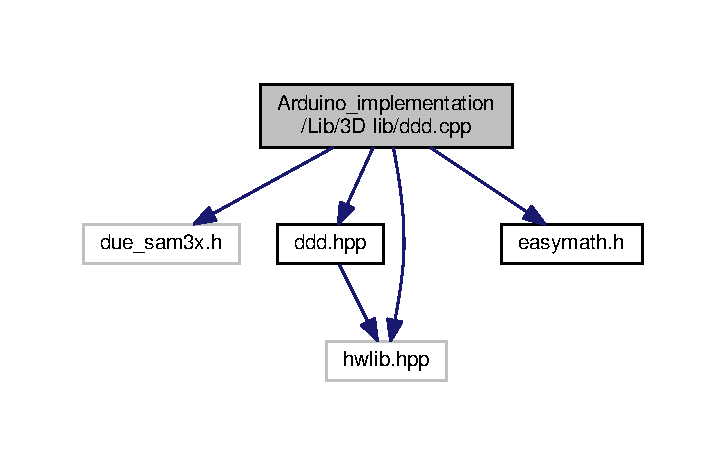
\includegraphics[width=349pt]{ddd_8cpp__incl}
\end{center}
\end{figure}


\subsection{Detailed Description}
\begin{DoxyAuthor}{Author}
Jan Halsema 
\end{DoxyAuthor}
\begin{DoxyCopyright}{Copyright}
Copyright (c) 2016, Jan Halsema 
\end{DoxyCopyright}

\hypertarget{ddd_8hpp}{\section{Arduino\+\_\+implementation/\+Lib/3\+D lib/ddd.hpp File Reference}
\label{ddd_8hpp}\index{Arduino\+\_\+implementation/\+Lib/3\+D lib/ddd.\+hpp@{Arduino\+\_\+implementation/\+Lib/3\+D lib/ddd.\+hpp}}
}


3\+D header.  


{\ttfamily \#include \char`\"{}hwlib.\+hpp\char`\"{}}\\*
Include dependency graph for ddd.\+hpp\+:
\nopagebreak
\begin{figure}[H]
\begin{center}
\leavevmode
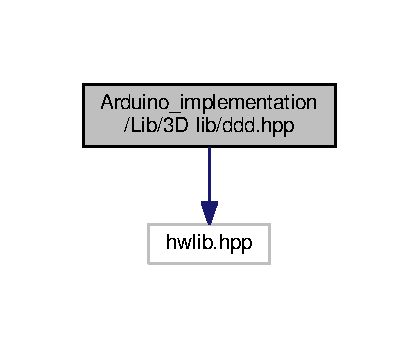
\includegraphics[width=201pt]{ddd_8hpp__incl}
\end{center}
\end{figure}
This graph shows which files directly or indirectly include this file\+:
\nopagebreak
\begin{figure}[H]
\begin{center}
\leavevmode
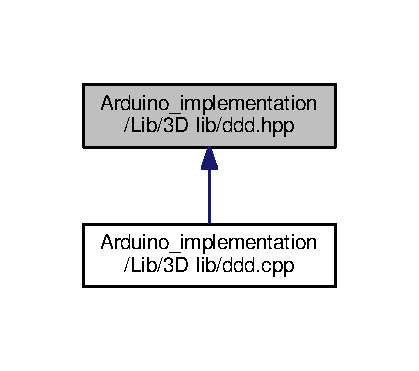
\includegraphics[width=201pt]{ddd_8hpp__dep__incl}
\end{center}
\end{figure}
\subsection*{Data Structures}
\begin{DoxyCompactItemize}
\item 
struct \hyperlink{structVertex}{Vertex}
\begin{DoxyCompactList}\small\item\em \hyperlink{structVertex}{Vertex} structure to store 3\+D coordinates. \end{DoxyCompactList}\item 
struct \hyperlink{structEdge}{Edge}
\begin{DoxyCompactList}\small\item\em \hyperlink{structEdge}{Edge} struct to connect 2 Vertexes. \end{DoxyCompactList}\item 
class \hyperlink{classdriedobj}{driedobj}
\begin{DoxyCompactList}\small\item\em The main class, it can manipulate and draw 3d objects. \end{DoxyCompactList}\end{DoxyCompactItemize}


\subsection{Detailed Description}
3\+D header. 

\begin{DoxyAuthor}{Author}
Jan Halsema 
\end{DoxyAuthor}
\begin{DoxyCopyright}{Copyright}
Copyright (c) 2016, Jan Halsema 
\end{DoxyCopyright}

\hypertarget{hwlib-dubblebufferd_8hpp}{\section{Arduino\+\_\+implementation/\+Lib/\+Dubblebufferlib/hwlib-\/dubblebufferd.hpp File Reference}
\label{hwlib-dubblebufferd_8hpp}\index{Arduino\+\_\+implementation/\+Lib/\+Dubblebufferlib/hwlib-\/dubblebufferd.\+hpp@{Arduino\+\_\+implementation/\+Lib/\+Dubblebufferlib/hwlib-\/dubblebufferd.\+hpp}}
}


Double bufferd Hwlib header, can be used as an extension to hwlib.  


{\ttfamily \#include $<$hwlib-\/graphics.\+hpp$>$}\\*
Include dependency graph for hwlib-\/dubblebufferd.hpp\+:
\nopagebreak
\begin{figure}[H]
\begin{center}
\leavevmode
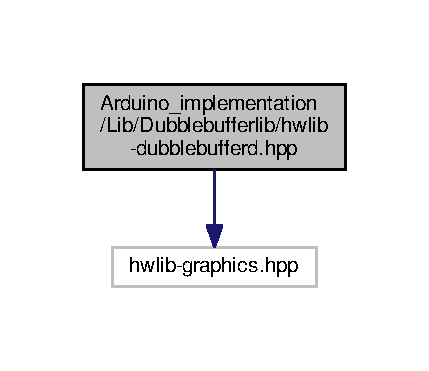
\includegraphics[width=206pt]{hwlib-dubblebufferd_8hpp__incl}
\end{center}
\end{figure}
\subsection*{Data Structures}
\begin{DoxyCompactItemize}
\item 
class \hyperlink{classhwlib_1_1bufferwindow}{hwlib\+::bufferwindow}
\begin{DoxyCompactList}\small\item\em the main class of dubblebufferd, a decorator for hwlib windows. \end{DoxyCompactList}\end{DoxyCompactItemize}


\subsection{Detailed Description}
Double bufferd Hwlib header, can be used as an extension to hwlib. 

\begin{DoxyAuthor}{Author}
Jan Halsema 
\end{DoxyAuthor}
\begin{DoxyCopyright}{Copyright}
Copyright (c) 2016, Jan Halsema 
\end{DoxyCopyright}

\hypertarget{easymath_8h}{\section{Arduino\+\_\+implementation/\+Lib/\+Mathlib/easymath.h File Reference}
\label{easymath_8h}\index{Arduino\+\_\+implementation/\+Lib/\+Mathlib/easymath.\+h@{Arduino\+\_\+implementation/\+Lib/\+Mathlib/easymath.\+h}}
}


My optimized math library, greatly inspired and influenced by the work of Oscar Liang and the Speed\+Trig math library.  


This graph shows which files directly or indirectly include this file\+:
\nopagebreak
\begin{figure}[H]
\begin{center}
\leavevmode
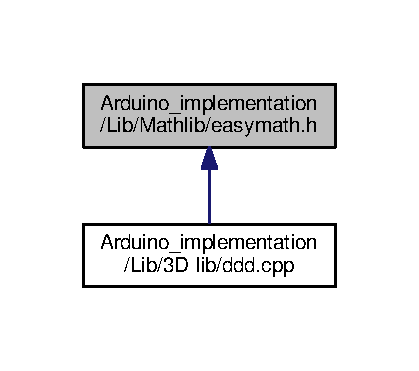
\includegraphics[width=201pt]{easymath_8h__dep__incl}
\end{center}
\end{figure}
\subsection*{Macros}
\begin{DoxyCompactItemize}
\item 
\hypertarget{easymath_8h_ab1fb5556708bdfa9e495e77c26b83b49}{\#define {\bfseries M\+A\+X\+\_\+\+U\+I\+N\+T}~65535}\label{easymath_8h_ab1fb5556708bdfa9e495e77c26b83b49}

\item 
\hypertarget{easymath_8h_a91a4a7c68f549b5f31dbced70ae07ee6}{\#define {\bfseries M\+I\+N\+\_\+\+I\+N\+T}~-\/32768}\label{easymath_8h_a91a4a7c68f549b5f31dbced70ae07ee6}

\item 
\hypertarget{easymath_8h_aaa1ac5caef84256eaeb39594e58e096f}{\#define {\bfseries M\+A\+X\+\_\+\+I\+N\+T}~32767}\label{easymath_8h_aaa1ac5caef84256eaeb39594e58e096f}

\item 
\hypertarget{easymath_8h_a7d0fbb86bc9c36a24b68f1a86bd61500}{\#define {\bfseries D\+E\+C1}~10}\label{easymath_8h_a7d0fbb86bc9c36a24b68f1a86bd61500}

\item 
\hypertarget{easymath_8h_a5daf9a5d8f55f52b92d5d8622fcc37ef}{\#define {\bfseries D\+E\+C2}~100}\label{easymath_8h_a5daf9a5d8f55f52b92d5d8622fcc37ef}

\item 
\hypertarget{easymath_8h_a8da9c4422fb27cc169f755221c465b8f}{\#define {\bfseries D\+E\+C3}~1000}\label{easymath_8h_a8da9c4422fb27cc169f755221c465b8f}

\item 
\hypertarget{easymath_8h_a9edfe1dccdb7b44e22be4c1fd0461f68}{\#define {\bfseries D\+E\+C4}~10000}\label{easymath_8h_a9edfe1dccdb7b44e22be4c1fd0461f68}

\end{DoxyCompactItemize}
\subsection*{Functions}
\begin{DoxyCompactItemize}
\item 
\hypertarget{easymath_8h_a989878f2df0f9bc4b679f6f635b03a65}{int {\bfseries float\+To\+Int} (float input)}\label{easymath_8h_a989878f2df0f9bc4b679f6f635b03a65}

\item 
\hypertarget{easymath_8h_a1d55e956d248733ed59d73d1af4c4f4c}{int {\bfseries rad\+To\+Micro} (float rad)}\label{easymath_8h_a1d55e956d248733ed59d73d1af4c4f4c}

\item 
float \hyperlink{easymath_8h_a1adb8c4358affb9f0af8a2595fa760b2}{sin} (int deg)
\item 
\hypertarget{easymath_8h_a515022cf3a12cae4d0431aa7f0b59ead}{float {\bfseries cos} (int deg)}\label{easymath_8h_a515022cf3a12cae4d0431aa7f0b59ead}

\item 
float \hyperlink{easymath_8h_a126f6bb9add8a4eb8e88937a0cc30ced}{acos} (float num)
\end{DoxyCompactItemize}
\subsection*{Variables}
\begin{DoxyCompactItemize}
\item 
\hypertarget{easymath_8h_aa08a577393243b86dfd2a97e61443673}{const float {\bfseries P\+I} = 3.\+13159265358979}\label{easymath_8h_aa08a577393243b86dfd2a97e61443673}

\item 
\hypertarget{easymath_8h_aed3c8a905ced968c76571c684553a46e}{const float {\bfseries P\+Iby2} = P\+I / 2}\label{easymath_8h_aed3c8a905ced968c76571c684553a46e}

\item 
const float \hyperlink{easymath_8h_af0d4961c00d407529a4a50ef9349a322}{S\+I\+N\+\_\+\+T\+A\+B\+L\+E} \mbox{[}181\mbox{]}
\item 
const byte \hyperlink{easymath_8h_a68aa53d757bb93d1364f9373ca84eb86}{A\+C\+O\+S\+\_\+\+T\+A\+B\+L\+E} \mbox{[}278\mbox{]}
\end{DoxyCompactItemize}


\subsection{Detailed Description}
My optimized math library, greatly inspired and influenced by the work of Oscar Liang and the Speed\+Trig math library. 

\begin{DoxyAuthor}{Author}
Jan Halsema 
\end{DoxyAuthor}
\begin{DoxyCopyright}{Copyright}
Copyright (c) 2016, Jan Halsema 
\end{DoxyCopyright}


\subsection{Function Documentation}
\hypertarget{easymath_8h_a126f6bb9add8a4eb8e88937a0cc30ced}{\index{easymath.\+h@{easymath.\+h}!acos@{acos}}
\index{acos@{acos}!easymath.\+h@{easymath.\+h}}
\subsubsection[{acos}]{\setlength{\rightskip}{0pt plus 5cm}float acos (
\begin{DoxyParamCaption}
\item[{float}]{num}
\end{DoxyParamCaption}
)}}\label{easymath_8h_a126f6bb9add8a4eb8e88937a0cc30ced}
The acos function uses a lookup table for corresponding output. Output data are stored as byte values (0 -\/ 255), they are scaled down to float number (0.\+0 -\/ 1.\+0) for output. \hypertarget{easymath_8h_a1adb8c4358affb9f0af8a2595fa760b2}{\index{easymath.\+h@{easymath.\+h}!sin@{sin}}
\index{sin@{sin}!easymath.\+h@{easymath.\+h}}
\subsubsection[{sin}]{\setlength{\rightskip}{0pt plus 5cm}float sin (
\begin{DoxyParamCaption}
\item[{int}]{deg}
\end{DoxyParamCaption}
)}}\label{easymath_8h_a1adb8c4358affb9f0af8a2595fa760b2}
The functions for sin and cos use lookup table to determine the sin or cos value of the input angle. Input for these functions are scaled up 10 times. e.\+g. -\/450 = -\/45.\+0 deg
\begin{DoxyItemize}
\item Both functions return a value between -\/1 and 1. (e.\+g. input\+: -\/450, output -\/$>$ -\/0.\+7071) 
\end{DoxyItemize}

\subsection{Variable Documentation}
\hypertarget{easymath_8h_a68aa53d757bb93d1364f9373ca84eb86}{\index{easymath.\+h@{easymath.\+h}!A\+C\+O\+S\+\_\+\+T\+A\+B\+L\+E@{A\+C\+O\+S\+\_\+\+T\+A\+B\+L\+E}}
\index{A\+C\+O\+S\+\_\+\+T\+A\+B\+L\+E@{A\+C\+O\+S\+\_\+\+T\+A\+B\+L\+E}!easymath.\+h@{easymath.\+h}}
\subsubsection[{A\+C\+O\+S\+\_\+\+T\+A\+B\+L\+E}]{\setlength{\rightskip}{0pt plus 5cm}const byte A\+C\+O\+S\+\_\+\+T\+A\+B\+L\+E\mbox{[}278\mbox{]}}}\label{easymath_8h_a68aa53d757bb93d1364f9373ca84eb86}
{\bfseries Initial value\+:}
\begin{DoxyCode}
= \{
  255, 254, 252, 251, 250, 249, 247, 246, 245, 243, 242, 241, 240, 238, 237, 236, 234, 233, 232, 231, 229, 
      228, 227, 225, 224, 223,
  221, 220, 219, 217, 216, 215, 214, 212, 211, 210, 208, 207, 206, 204, 203, 201, 200, 199, 197, 196, 195, 
      193, 192, 190, 189, 188,
  186, 185, 183, 182, 181, 179, 178, 176, 175, 173, 172, 170, 169, 167, 166, 164, 163, 161, 160, 158, 157, 
      155, 154, 152, 150, 149,
  147, 146, 144, 142, 141, 139, 137, 135, 134, 132, 130, 128, 127, 125, 123, 121, 119, 117, 115, 113, 111, 
      109, 107, 105, 103, 101,
  98, 96, 94, 92, 89, 87, 84, 81, 79, 76, 73, 73, 73, 72, 72, 72, 71, 71, 71, 70, 70, 70, 70, 69, 69, 69, 
      68, 68, 68, 67, 67, 67,
  66, 66, 66, 65, 65, 65, 64, 64, 64, 63, 63, 63, 62, 62, 62, 61, 61, 61, 60, 60, 59, 59, 59, 58, 58, 58, 
      57, 57, 57, 56, 56, 55,
  55, 55, 54, 54, 53, 53, 53, 52, 52, 51, 51, 51, 50, 50, 49, 49, 48, 48, 47, 47, 47, 46, 46, 45, 45, 44, 
      44, 43, 43, 42, 42, 41,
  41, 40, 40, 39, 39, 38, 37, 37, 36, 36, 35, 34, 34, 33, 33, 32, 31, 31, 30, 29, 28, 28, 27, 26, 25, 24, 
      23, 23, 23, 23, 22, 22,
  22, 22, 21, 21, 21, 21, 20, 20, 20, 19, 19, 19, 19, 18, 18, 18, 17, 17, 17, 17, 16, 16, 16, 15, 15, 15, 
      14, 14, 13, 13, 13, 12,
  12, 11, 11, 10, 10, 9, 9, 8, 7, 6, 6, 5, 3, 0
\}
\end{DoxyCode}
The acos lookup table is split into three parts, which has a higher accuracy closer to acos(1).
\begin{DoxyItemize}
\item 0 to 0.\+9 is in steps of 0.\+0079 rads. (1/127)
\item 0.\+9 to 0.\+99 is in steps of 0.\+0008 rads. (0.\+01/127)
\item 0.\+99 to 1 is in steps of 0.\+0002 rads. (0.\+01/64) 
\end{DoxyItemize}\hypertarget{easymath_8h_af0d4961c00d407529a4a50ef9349a322}{\index{easymath.\+h@{easymath.\+h}!S\+I\+N\+\_\+\+T\+A\+B\+L\+E@{S\+I\+N\+\_\+\+T\+A\+B\+L\+E}}
\index{S\+I\+N\+\_\+\+T\+A\+B\+L\+E@{S\+I\+N\+\_\+\+T\+A\+B\+L\+E}!easymath.\+h@{easymath.\+h}}
\subsubsection[{S\+I\+N\+\_\+\+T\+A\+B\+L\+E}]{\setlength{\rightskip}{0pt plus 5cm}const float S\+I\+N\+\_\+\+T\+A\+B\+L\+E\mbox{[}181\mbox{]}}}\label{easymath_8h_af0d4961c00d407529a4a50ef9349a322}
{\bfseries Initial value\+:}
\begin{DoxyCode}
=\{
  0.000000, 0.008727, 0.017452, 0.026177, 0.034899, 0.043619, 0.052336, 0.061049, 0.069756, 0.078459, 0.087
      156, 0.095846, 0.104528,
  0.113203, 0.121869, 0.130526, 0.139173, 0.147809, 0.156434, 0.165048, 0.173648, 0.182236, 0.190809, 0.199
      368, 0.207912, 0.216440,
  0.224951, 0.233445, 0.241922, 0.250380, 0.258819, 0.267238, 0.275637, 0.284015, 0.292372, 0.300706, 0.309
      017, 0.317305, 0.325568,
  0.333807, 0.342020, 0.350207, 0.358368, 0.366501, 0.374607, 0.382683, 0.390731, 0.398749, 0.406737, 0.414
      693, 0.422618, 0.430511,
  0.438371, 0.446198, 0.453990, 0.461749, 0.469472, 0.477159, 0.484810, 0.492424, 0.500000, 0.507538, 0.515
      038, 0.522499, 0.529919,
  0.537300, 0.544639, 0.551937, 0.559193, 0.566406, 0.573576, 0.580703, 0.587785, 0.594823, 0.601815, 0.608
      761, 0.615661, 0.622515,
  0.629320, 0.636078, 0.642788, 0.649448, 0.656059, 0.662620, 0.669131, 0.675590, 0.681998, 0.688355, 0.694
      658, 0.700909, 0.707107,
  0.713250, 0.719340, 0.725374, 0.731354, 0.737277, 0.743145, 0.748956, 0.754710, 0.760406, 0.766044, 0.771
      625, 0.777146, 0.782608,
  0.788011, 0.793353, 0.798636, 0.803857, 0.809017, 0.814116, 0.819152, 0.824126, 0.829038, 0.833886, 0.838
      671, 0.843391, 0.848048,
  0.852640, 0.857167, 0.861629, 0.866025, 0.870356, 0.874620, 0.878817, 0.882948, 0.887011, 0.891007, 0.894
      934, 0.898794, 0.902585,
  0.906308, 0.909961, 0.913545, 0.917060, 0.920505, 0.923880, 0.927184, 0.930418, 0.933580, 0.936672, 0.939
      693, 0.942641, 0.945519,
  0.948324, 0.951057, 0.953717, 0.956305, 0.958820, 0.961262, 0.963630, 0.965926, 0.968148, 0.970296, 0.972
      370, 0.974370, 0.976296,
  0.978148, 0.979925, 0.981627, 0.983255, 0.984808, 0.986286, 0.987688, 0.989016, 0.990268, 0.991445, 0.992
      546, 0.993572, 0.994522,
  0.995396, 0.996195, 0.996917, 0.997564, 0.998135, 0.998630, 0.999048, 0.999391, 0.999657, 0.999848, 0.999
      962, 1.000000
\}
\end{DoxyCode}
The sin lookuptable. 
%--- End generated contents ---

% Index
\newpage
\phantomsection
\addcontentsline{toc}{chapter}{Index}
\printindex

\end{document}
